\documentclass[a4paper]{article}
\usepackage[english]{babel}
\usepackage{graphicx}
\usepackage[utf8]{inputenc}
\usepackage[T1]{fontenc}
\usepackage[us]{datetime}
\usepackage{multirow}
\usepackage{caption}
\usepackage{amsmath}
\usepackage{amsthm}
\usepackage{tocloft}
\usepackage[nottoc]{tocbibind}
\usepackage{amssymb}
\usepackage{caption}
\captionsetup[figure]{labelfont=bf}
\captionsetup[table]{labelfont=bf}
\usepackage{float}
\usepackage{bbm}
\usepackage{theoremref}
\usepackage{setspace}
\captionsetup[figure]{labelfont=bf}
%% Theorems
\newtheorem{prop}{Proposition}
\newtheorem*{remark}{Remark}
%%


\begin{document}

\begin{titlepage}
\begin{center}

\large \textbf{Semesterthesis}

\vspace{1cm}
\hrule
\vspace{0.4cm}
\huge \textbf{Implementation of multi-asset spread option pricing methods}\\
\vspace{0.4cm}
\hrule
\vspace{0.4cm}
\textsc{\large ETH Z\"urich}\\
\vspace{0.4cm}
\large {November 2015}

\vspace{6cm}




\vspace{4cm}
\large \emph{Author:}\\
\large Daniel W\"alchli\\
\large wadaniel@student.ethz.ch\\
\vspace{1cm}
\noindent
\begin{minipage}{0.4\textwidth}
\begin{flushleft} \normalsize
\emph{Examiner:}\\
Prof. Dr. Erich \textsc{Farkas}\\
PLE-H05\\
Plattenstrasse 22\\
8032 Z\"urich\\
farkas@math.ethz.ch
\end{flushleft}
\end{minipage}%
\begin{minipage}{0.4\textwidth}
\begin{flushright} \normalsize
\emph{Supervisor:} \\
Mrs. Fulvia \textsc{Fringuellotti}\\
PLE-G07\\
Plattenstrasse 22\\
8032 Z\"urich\\
fulvia.fringuellotti@bf.uzh.ch
\end{flushright}
\end{minipage}

\end{center}
\end{titlepage}

\pagenumbering{roman}
\setcounter{page}{1}
\section*{Abstract}
I analyse two approximation methods for pricing European basket-spread options: the second-order boundary approximation introduced by S.Deng, M.Li, and J.Zhou \cite{sob} and the hybrid moment matching method associated to the improved comonotonic upper bound presented by G.Deelstra, A.Petkovic and M.Vanmaele \cite{hybmmicub}. Both method are considered to be very fast and accurate. I present both methods and compare their relative performances based on my MATLAB implementation. In the performance analysis I use several pricing examples to report on the accuracy of both methods. 

\newpage

\renewcommand{\cftsecleader}{\cftdotfill{\cftdotsep}}
\tableofcontents

\newpage
\pagenumbering{arabic}
\setcounter{page}{1}
\section{Introduction}
A European basket-spread option is a financial derivative, whose
maturity is given by the difference (the so called spread) between two 
baskets of aggregated and weighted underlying asset prices. In mathematical terms it's payoff is given by 
the formula:
\begin{equation}
\label{eq:po}
P(S,T) = (\sum_{i=0}^M w_iS_i(T) - \sum_{j=M+1}^{M+N} w_jS_j(T) - K)^+,
\end{equation}
with $(x)^+=max(x,0)$ and where $S_i$ is the ith underlying asset price, $w_i$ its weight and $K$ is the strike price.
Basket-spread options play an important role in hedging a portfolio of correlated long and short
positions. Especially they are very common in commodity markets,
as producers are exposed to risks arising from spreads between feedstock and end products.
Basket-spread options are traded over-the-counter and on exchanges. Since there is no
closed-form solution available for the fair price it is inescapable to have an accurate and
fast approximation method at hand. The multi-dimensionality and
hence the lack of a marginal distribution for the basket-spread makes it impossible to give an exact
analytical representation for the price (even not in the simplest framework
where the asset prices are driven by  correlated geometric Brownian motions). Numerical approaches such 
as Monte Carlo simulations or PDE methods become very slow and hence inpracticable as the number of underlyings increases. 
Therefore I closely look at two different basket-spread option pricing methods which have been 
introduced by S.Deng, M.Li, and J.Zhou \cite{sob} and by G.Deelstra, A.Petkovic and M.Vanmaele \cite{hybmmicub}. According to the authors both the second-order boundary approximation method [1,Chap.3,Prop.5] and the hybrid moment matching method associated to the improved comonotonic upper bound (HybMMICUB)
[2,Chap.3,Prop.5] are considered to be extremely fast and accurate. Therefore I implement both methods in MATLAB
and compare their numerical performances as a function of the basket-spread characteristics. 
As a comparison benchmark I estimate the true prices with Monte Carlo simulations also implemented in MATLAB.\\
The paper is organized as follows. In section 2 I first show the assumptions on which both methods are based on. Then I present the underlying theories for both the  SOB method and the HybMMICUB method.\\
In section three I start with a short statement about the numerical experiments I am using to test my implementations. Then I explain the computational bottlenecks of both methods and look at their computing time. Last I discuss my numerical experiments.

\newpage
\section{Approximation methods}
\label{sec:am}
In the next subsection (\ref{sec:ms}) I show the assumptions on which both the second-order boundary method and the HybMMICUB method are based on. In teh following two subsections I formally present both approximation methods. These subsections closely follow the works of S.Deng, M.Li, and J.Zhou \cite{sob} and by G.Deelstra, A.Petkovic and M.Vanmaele \cite{hybmmicub}.

\subsection{Model setup}
\label{sec:ms}
Consider M+N assets $S_1(t), S_2(t), ...,$ and $S_{M+N}(t)$ each of it following a geometric Brownian motion
$$dS_i(t) = u_iS_i(t)dt + \sigma_iS_i(t)dW_i(t).$$
The correlations of the Brownian motions $W_i(t)$ is given by the matrix $\varrho=(\rho_{i,j})$. 
The payoff of the European basket-spread has already been introduced in equation \ref{eq:po}. Conditioning on the initial asset price $S_i(0), log(S_i(T))$ is jointly normally distributed with mean $\mu_i$, variance $\sigma_i^2$ and correlation matrix $\rho_{i,j}$ for i,j = 1,2,...,M+N. 
Further the interest rate $r$ is constant and the price of the European basket-spread option is given by
\begin{equation}
\label{eq:mg}
V = e^{-rT}\mathbb{E}^{\mathbb{Q}}[(\sum_{i=0}^M w_iS_i(T) - \sum_{j=M+1}^{M+N} w_jS_j(T) - K)^+],
\end{equation}
where $\mathbb{Q}$ is the risk-neutral measure under which discounted security prices are martingales.
In the geometric brownian motion (GBM) setting the means and variances are defined by 
\begin{equation}
\mu_i = E^\mathbb{Q}[log(S_i(T))] = log(S_i(0)) + (r-\frac{1}{2}{\sigma_k}^2)T
\end{equation}
and
\begin{equation}
{\sigma_i}^2 = Var^\mathbb{Q}[log(S_k(T))] = \sigma_i\sqrt{T}, \quad i=1,2,...,M+N.
\end{equation}
Because the weights $w_i$ can be incorporated in the asset price by taking $S_i(t)'=w_iS_i(t)$ and $\mu_i=log(w_i)+\mu_i, \sigma_i'=\sigma_i$ and $\rho_{i,j}'=\rho_{i,j},$ I will assume that all weights $w_i$ equal 1 without loss of generality.

\subsection{Second-order Boundary Method}
\label{sec:sob}
The second-order boundary method for two-asset spread options (SOB) has been introduced in 2006 by Deng, Li and Zhou \cite{sob2} and it was extended in 2007 to the multi-asset case \cite{sob}. Beside the SOB method Deng, Li and Zhou also introduced the extended Kirk approximation in \cite{sob}. Their work is a valuable contribution because numerous methods have been existing for spread options involving only two underlyings. In \cite{sob} Deng, Li and Zhou compare their two methods with a pricing method from Carmona and Durrleman (2005) \cite{cd} which also approximates the value of a multi-asset spread option. In \cite{sob} they conclude that the SOB method is the most accurate and also the fastest. The computational edge of the SOB method lies in its closed form solution which involves solely arithmetic calculations.\\
The SOB method approximates the price of a spread option with payoff
\begin{equation}
\label{eq:sobpo}
(S_0(T) - \sum_{j=1}^{N}S_j(T) - K)^+, 
\end{equation}
thus we introduce the random variables 
$$H_0(t)=\sum_{i=1}^M S_t(t)$$ 
and 
$$H_k(t)=S_{k+M}(t), \quad k=1,2,...,N$$
which can be plugged into preceding payoff (equation \ref{eq:sobpo}) and replace $S_0(T)$ and $S_j(T)$. The idea is to approximate the distribution of $H_0(T)$ by the geometric averages of the corresponding  $S_i$'s to extend the SOB method in order to price basked-spread options. Notice that $log(H_0(T))$ is not normally distributed nor are the $log(H_i)$'s jointly normally distributed. This comes from the fact that the sum of lognormal distributed random variables is no longer lognormal distributed.\\
The mean and the variance of the newly introduced random variable $H_0(T)$ is approximated by 
\begin{equation}
\mu_0^H = log(\sum_{i=0}^{M}e^{\mu_i+1/2{\sigma_i}^2}) - 1/2{\sigma_0^H}^2
\end{equation}
\begin{equation}
\sigma_0^H=\frac{1}{M}\sqrt{\sum_{i=1}^M \sum_{j=1}^M \rho_{i,j} \sigma_i \sigma_j}
\end{equation}
Next we define random variables $X$ and $Y_k$ by
$$X = \frac{log(H_0(T))-\mu_0^H}{\sigma_0^H}, Y_k = \frac{log(H_k(T))-\mu_k^H)}{\sigma_k^H}, \quad k=1,2,...,N$$
whereas $\mu_k^H = \mu_k+M$ and $\sigma_k^H = \sigma_k+M$ for $k=1,2,...,N$. Following that we can approximate the variables $X$ and $Y_k$ as jointly normally distributed with mean vector 0, variance vector 1 and correlation matrix $\Sigma = (q_{i,j})$ for $i,j=0,1,...,N$, where 
$$q_{0,0}=1,$$ 
$$q_{0,k}=q_{k,0}=1,$$
$$q_{i,j}=\rho_{M+i,M+j}.$$
Rewriting the correlation matrix $\Sigma$ as a composition of a Nx1 vector $\Sigma_{10}$ and $\Sigma_{11}$ the NxN correlation matrix of the $Y_k$'s simplifies notation for later computations:
$$\Sigma = (q_{i,j}) = \begin{pmatrix} 1 & \Sigma_{10}' \\ \Sigma_{10} & \Sigma_{11} \end{pmatrix}.$$ 
Before introducing the methods for valuing basket-spread option a short analysis of the exercise boundary is necessary. At time T, the  basket-spread option is in-the-money 
if $H_0(T) - \sum_{k=1}^N S_k(T)-K>0$. If $K>0$, rewriting this inequality in terms of the random variable $X$ gives
$$X>\frac{log(\sum e^{\sigma_kY_k-\mu_k+K}-\mu_0^H)}{\sigma_0^H}$$
Conditioned on $Y_k=y_k$, the option is in-the-money if $X>x(y)$, where
$$x(y)\equiv\frac{log(\sum e^{\sigma_ky_k-\mu_k+K}-\mu_0^H)}{\sigma_0^H}.$$
Note that the exercise boundary $x(y)$ is a nonlinear function in the components of y but close to being linear around $y=0$.
The analytical computation of the expectation value given in equation \ref{eq:mg} is shown below:
\begin{equation}
\label{eq:val}
V= e^{-rT} \int_{\mathbb{R}^N} \int_\mathbb{R} \big(e^{\sigma_0^Hx+\mu_0^H}-\sum_{k=1}^Ne^{\sigma_ky_k+\mu_k}-K\big)^+\phi(\{x,y\};0,\Sigma) dx dy,
\end{equation}
whereas $\phi(z;m;\Sigma)$ stands for the multivariate normal density function with mean vector m and covariance matrix $\Sigma$. Note that the random variables $X$ and $Y$ in equation $\ref{eq:val}$ are approximately jointly normally distributed with density $\phi({x,y};0;\Sigma)$.\\
Proposition 1 (Pearson (1995) [5]) allows us to reduce the (N+1)-dimensional integral from above (equation \ref{eq:val}) to N+2 N-dimensional integrals.

\begin{prop}
\label{prop:price}
Under the jointly-normal returns setup with $K \geq 0$ and det $\Sigma \neq 0$, the price of the spread option (equation \ref{eq:sobpo}) can be written as
$$V=e^{-rT+\mu_0^H+\frac{1}{2}\sigma_0^{H2}}I_0-\sum_{k=1}^Ne^{-rT+\mu_k+\frac{1}{2}\sigma_k^2}I_k-Ke^{-rT}I_{N+1}.$$
The integrals $I_i$'s are given by
$$I_0=\int_{\mathbb{R}^N}\phi(y;0,\Sigma_{11})\Phi\big(A(y+\sigma_0^H\Sigma_{10})+\sigma_0^H\sqrt{\Sigma_{x|y}}\big)dy,$$
$$I_k=\int_{\mathbb{R}^N}\phi(y;0,\Sigma_{11})\Phi\big(A(y+\sigma_k\Sigma_{11}e_k)\big)dy, \quad k=1,2,...,N,$$
$$I_{N+1}=\int_{\mathbb{R}^N}\phi(y;0,\Sigma_{11})\Phi\big(A(y)\big)dy,$$
where $e_k$ is the unit column vector (0,...,0,1,0,...,0)' with 1 at the k-th position, and
$$A(y)=\frac{\mu_{x|y}-x(y)}{\sqrt{\Sigma_{x|y}}},$$
with
\begin{equation}
\label{eq:inv}
\mu_{x|y}=\Sigma_{10}'\Sigma_{11}^{-1}y, \quad \Sigma_{x|y}=1-\Sigma_{10}'\Sigma_{11}^{-1}\Sigma_{10}.
\end{equation}
\end{prop}

In proposition \ref{prop:price}, $\Phi(z)$ stands for the one-dimensional cumulative distribution function. Note that I already plugged in the approximated mean $\mu_0^H$ and variance $\sigma_0^H$ of the random variable $H_0(t)$ instead of the mean and variance of $S_0(t)$. From now one I'll be working with the approximations $\mu_0^H$ and $\sigma_0^H$.\\
Keep in mind that det $\Sigma \neq 0$ such that $\Sigma_{x|y} \neq 0$, det $\Sigma_{11} \neq 0$ and $A(y)$ is always well defined. In the GBM setting, the price $V$ reduces to the form
\begin{equation}
\label{eq:cf}
V = S_0(t)e^{-q_0T}I_0-\sum_{k=1}^NS_k(0)e^{-q_kT}I_k-Ke^{-rT}I_{N+1}.
\end{equation}
The proof of proposition 1 can be found in [1] in the appendix. 
The formula presented above is the starting point of the next approximation step. A second order taylor expansion of the exercise boundary $x(y)$ and the function $A(y)$ allows to compute $I_k$'s in closed form. Observe that $A(y)$ is also close to being linear around $y=0$. The second order approximation of $x(y)$ and $A(y)$ is given by proposition \ref{prop:approx}:

\begin{prop}
\label{prop:approx}
The exercise boundary x(y) can be approximated to second order in y as
\begin{equation}
x(y)\approx x(0)+\triangledown x|_0'y+\frac{1}{2}y'\triangledown^2x|_0y,
\end{equation}
where
\begin{equation}
x(0)=\frac{log(R+K)-\mu_0^H}{\sigma_0^H},
\end{equation}
\begin{equation}
(\triangledown x|_0)_k=\frac{e^{\mu_k}\sigma_k}{\sigma_0^H(R+K)},k=1,2,...,N,
\end{equation}
\begin{equation}
(\triangledown^2 x|_0)_{i,j}=\frac{e^{\mu_i+\mu_j}\sigma_i\sigma_j}{\sigma_0^H(R+K)^2}+\delta_{i,j}\frac{v_j^2e^\mu_j}{\sigma_0^H(R+K)},i,j=1,2,...,N
\end{equation}
with $\delta_{i,j}$ being the Kronecker delta function, and
\begin{equation}
R=\sum_{k=1}^Ne^{\mu_k}.
\end{equation}
Accordingly, the function A(y) can be approximated as
\begin{equation}
A(y)=\frac{\mu_{x|y}-x(y)}{\sqrt{\Sigma_{x|y}}}\approx c+d'y+y'Ey,
\end{equation}
where
\begin{equation}
c=-\frac{log(R+K)-\mu_0^H}{v_0^H\sqrt{\Sigma_{x|y}}},
\end{equation}
\begin{equation}
d=\frac{1}{\sqrt{\Sigma_{x|y}}}(\Sigma_{11}^{-1}\Sigma_{10}-\triangledown x|_0),
\end{equation}
\begin{equation}
E=-\frac{1}{2\sqrt{\Sigma_{x|y}}}(\triangledown^2 x|_0).
\end{equation}
\end{prop}
To gain a closed-form approximation of the option price (equation \ref{eq:cf}) we need to further expand $\Phi(c+d'y+y'Ey)$ into three terms to second order in $y'Ey$ around $y'Ey=\epsilon$. The approximation formula of the price of a basket-spread is presented in proposition \ref{prop:approx2}, which has been derived with the help of an identity presented by Li (2007) \cite{li}. 
\begin{prop}
\label{prop:approx2}
Let $K\geq0$ and $det \Sigma \neq 0$. The spread option price V under the general jointly-normal returns setup is given by
\begin{equation}
\label{eq:cf2}
V=e^{-rT+\mu_0^H+\frac{1}{2}\sigma_0^{H2}}I_0-\sum_{k=1}^Ne^{-rT+\mu_k+\frac{1}{2}\sigma_k^2}I_k-Ke^{-rT}I_{N+1}.
\end{equation}
The integrals $I_i$'s are approximated as
$$I_i\approx J^0(c_i,d_i)+J^1(c_i,d_i)-\frac{1}{2}J^2(c_i,d_i), i=0,1,...,N+1,$$
where the scalar functions $J^i$ are defined as
\begin{equation}
\label{eq:j0}
J^0(u,v)=\Phi\Big(\frac{u}{\sqrt{1+v'v}}\Big),
\end{equation}
\begin{equation}
\label{eq:j1}
J^1(u,v)=\frac{\lambda}{\sqrt{1+v'v}}\phi\Big(\frac{u}{\sqrt{1+v'v}}\Big),
\end{equation}
\begin{equation}
\label{eq:j2}
\begin{split}
J^2(u,v)=&\frac{u}{(1+v'v)^{3/2}}\phi\Big(\frac{u}{\sqrt{1+v'v}}\Big)\Big\{\lambda^2+2tr[(PFP)^2]- \\
	&4\lambda(1+v'v)(v'P^2FP^2v)+(4u^2-8-8v'v)||PFP^2v||^2\Big\},
\end{split}
\end{equation}
with
\begin{equation}
\label{eq:p}
P=P(v)\equiv(I+vv')^{-1/2},
\end{equation}
\begin{equation}
\lambda=\lambda(u,v)\equiv u^2v'P^2FP^2v+tr(PFP)-tr(F),
\end{equation}
where tr stands for the trace operator of a matrix. The scalars $c_i$, vectors $d_i$, and matrix $F$ are given by
\begin{equation}
c_0=c+tr(F)+\sigma_0^H\sqrt{\Sigma_{x|y}}+\sigma_0^H\Sigma_{10}'d+{\sigma_0^H}^2\Sigma_{10}'E\Sigma_{10},
\end{equation}
\begin{equation}
\label{eq:d0}
d_0=\Sigma_{11}^{1/2}(d+2\sigma_0^HE\Sigma_{10}),
\end{equation}
\begin{equation}
c_k=c+tr(F)+\sigma_ke_k'\Sigma_{11}d+\sigma_k^2e_k'\Sigma_{11}E\Sigma_{11}e_k,k=0,1,...,N,
\end{equation}
\begin{equation}
\label{eq:dk}
d_k=\Sigma_{11}^{1/2}(d+2\sigma_kE\Sigma_{11}e_k),k=1,2,...,N,
\end{equation}
\begin{equation}
c_{N+1}=c+tr(F),
\end{equation}
\begin{equation}
\label{eq:dN1}
d_{N+1}=\Sigma_{11}^{1/2}d,
\end{equation}
\begin{equation}
F=\Sigma_{11}^{1/2}E\Sigma_{11}^{1/2},
\end{equation}
with $\Sigma_{x|y}$ given in proposition \ref{prop:price}.
\end{prop}
The computation of equations \ref{eq:j0} - \ref{eq:j2} in proposition \ref{prop:approx2} appears to be cumbersome but it can be bypassed which is shown in proposition \ref{prop:app2short}. The proofs of propositions \ref{prop:approx2} and \ref{prop:app2short} can be found in the appendix of \cite{sob}. 
\begin{prop}
\label{prop:app2short}
With $P = P(v)$ as defined in equation \ref{eq:p}, we have
$$P=I-\theta vv', P^2=I-\psi vv',$$
where the scalars $\theta$ and $\psi$ are given by
\begin{equation}
\theta=\theta(v)=\frac{\sqrt{1+v'v}-1}{v'v+\sqrt{1+v'v}},\psi=\psi(v)=\frac{1}{1+v'v}.
\end{equation}
Furthermore, we have
$$tr[(PFP)^2]=tr(F^2)-\psi(1+\psi)v'F^2v,$$
$$v'P^2FP^2v=\psi^2v'Fv,$$
$$||PFP^2v||^2=\psi^2[v'F^2v-\psi(v'Fv)^2],$$
$$tr(PFP)=tr(F)-\psi v'Fv.$$
Thus the scalar function $J^i$'s given in (\ref{eq:j0}-\ref{eq:j2}) can be simplified as
\begin{equation}
J^0(u,v)=\Phi(u\sqrt{v}),
\end{equation}
\begin{equation}
J^1(u,v)=\psi^{3/2}(\psi u^2/1)v'Fv\phi(u\sqrt{\psi}),
\end{equation}
\begin{equation}
\begin{split}
J^2(u,v)=&u\psi^{3/2}\phi(u\sqrt{v})\big\{2tr(F^2) - 4(1-tr(F))\psi-\psi^2)v'Fv+ \\
	& \psi^2(9+(2-3u^2)\psi-u^2(4-u^2)\psi^2)(v'Fv)^2-\\
	&2\psi(5+(1-2u^2)\psi)v'F^2v\big\}.
\end{split}
\end{equation}
\end{prop}

\newpage
\subsection{Hybrid Moment Matching associated to Improved \\Comonotonic Upper Bound}
\label{sec:hybmmicup}
The hybrid moment matching method associated to improved comonotonic upper bound method (HybMMICUP) combines two approximation techniques. First, the underlyings are split up according their sign and aggregated in two sums 
$\mathbb{S}_1=\sum_{i=1}^MS_i$ and $\mathbb{S}_2=\sum_{j=M+1}^{M+N}S_j.$ Then both sums are moment matched with a log-normal random variable. Second, the price of the resulting spread option with payoff $(\mathbb{S}_1-\mathbb{S}_2-K)^+$ is approximated with the improved comonotonic upper bound method. Moment matching methods, the improved comonotonic upper bound and the HybMMICUP procedure have been presented by Deelstra, Petkovic and Vanmaele in 2009 [2]. The numerical results from [2] show that the HybMMICUP method  performs best at approximating the price of a basket-spread option. It can also price options of Asian type but this case won’t be treated in my work.\\
More formally, the fair value of the European basket-spread option will be rewritten as
\begin{equation}
\label{eq:spread}
V = e^{-rT}\mathbb{E}^\mathbb{Q}(\mathbb{S}_1(T) - \mathbb{S}_2(T) - K)^+, 
\end{equation} 
where $\mathbb{S}_j$ is a log-normal random variable with mean $u_j = 2ln(m_{1j}) - 1/2ln(m_{2j})$ and variance $\sigma_j^2 = ln(m_{2j})-2ln(m_{1j}).$
$S_1$ and $S_2$ represent the sums of the assets with positive and negative sign and $m_{1j}$ and $m_{2j}$ are the first and second moment of the respective sum $S_j$. There are several ways of approximating the moments of a sum of log-normal distributed random variables. The formulas I used in my implementation 
are
\begin{equation}
m_{11}=e^{rT}\sum_{i=1}^{M}S_i(0), \quad m_{12}=e^{rT}\sum_{i=M+1}^{M+N}S_i(0), 
\end{equation}
\begin{equation}
m_{2j}=e^{2rT}\sum_{i=1}^{M}\sum_{j=1}^{M+N}S_i(0)S_j(0)e^{\rho_{i,j}\sigma_i\sigma_jT}.
\end{equation}
To approximate the spread given in equation \ref{eq:spread} I additionally need the correlation coefficient $\rho$ of $ln(\mathbb{\tilde{S}}_1)$ and $ln(\mathbb{\tilde{S}}_2)$ . Note the tildes above $\mathbb{S}$ as we are left with moment matching approximations of log-normal random variables. The coefficient $\rho$ can be recovered from the equality of cross moments (crm):
$$\mathbb{E}[S_1S_2] = \mathbb{E}[\tilde{S}_1\tilde{S}_2],$$
namely
\begin{equation}
crm:=\sum_{i=1}^{M}\sum_{j=1}^{M+N}\mathbb{E}[S_i(T)S_j(T)]=e^{\mu_1+\mu_2+1/2\sigma_1^2+1/2\sigma_2^2+\sigma_1\sigma2\rho},
\end{equation}
where $\mathbb{E}[S_i(T)S_j(T)] = S_i(0) S_j(0) e^{2rT+\rho_{ij}\sigma_i\sigma_jT}.$\\
For an approximation of the spread (\ref{eq:spread}) the improved comonotonic upper bound (ICUB) is used. The ICUB is displayed in the next proposition, the proof and derivation can be found in [2]:
\begin{prop}
Consider the following stop-loss premium
$$\mathbb{E}[(e^{\mu_1+\sigma_1X_1}-e^{\mu_2+\sigma_2X_2}-K)^+],$$
with $X_1$, $X_2$ two correlated standard normal random variables. The comonotonic improved upper bound of this spread is given by
\begin{equation}
\label{eq:ints}
\begin{split}
V \simeq &\sum_{i=1}^2\epsilon_i\int_0^1e^{\mu_i+A_i(u)+1/2Y_i^2}\Phi\big(Y_i-\Phi^{-1}\big(F_{\mathbb{S}^{ic}|U=u}(K)\big)\big)du\\
	&-K\big(1-F_{\mathbb{S}^{ic}}(K)\big),
\end{split}
\end{equation}
where $\epsilon_1=1$ and $\epsilon_2=-1$, and where $F_{\mathbb{S}^{ic}|U=u}$ can be found by solving
\begin{equation}
\label{eq:fzero}
\sum_{i=1}^2\epsilon_ie^{\mu_i+A_i(u)+Y_i\Phi^{-1}(F_{\mathbb{S}^{ic}|U=u}(K))}=K,
\end{equation}
with, for $\gamma_i$ denoting the correlation between $X_i$ and the conditioning variable $\Lambda \stackrel{d}{=} \mathbb{E}[\Lambda]+\sigma_{\Lambda}\Phi^{-1}(U)$
\begin{equation*}
A_i(u)=\gamma_i\sigma_i\Phi^{-1}(u),\quad Y_i=\epsilon_i\sigma_i\sqrt{1-\gamma_i^2}, \quad F_{\mathbb{S}^{ic}}(K) = \int_0^1F_{\mathbb{S}^{ic}|U=u}(K)du.
\end{equation*}
\end{prop}
The corelation coefficient $\gamma_i$ is calculated as follows:
\begin{equation}
\gamma_i = \frac{e^{\mu_i}\sigma_i+e^{\mu_j}\sigma_j\rho}{\sqrt{e^{2\mu_1}\sigma_1^2+2e^{\mu_1+\mu_2}\sigma_1\sigma_2+e^{2\mu_2}\sigma_2^2}}.
\end{equation}
\begin{remark}
In the presentation of the HybMMICUP method I also omitted the weights of the assets as they can be incorporated in the price of each asset how indicated in subsection \ref{sec:ms}.
\end{remark}

\newpage
\section{Numerical Analysis}
\label{sec:na}
This section enlightens the computational bottlenecks, such as complexity and instabilities, of both the SOB and the HybMMICUB method. The analysis is based on my MATLAB implementations \emph{priceBasketSpreadOptionSOB.m} and \emph{priceBasketSpreadOptionHybMMICUB.m}.\\
I test my implementations within different settings, meaning I create artificial compositions of spot prices $S_k(0)$, variance vectors $\sigma$ and correlation matrices $\Sigma$. I use spot price vectors either of type \emph{charged} $S_c$ or of type \emph{descending} $S_d$ which I define as follows: 
$$S_{c}(0) = [10(N+1), 10, ..., 10],\quad S_{d}(0) = [10N, 10(N-1), ..., 10].$$  
The volatility vector is either of type \emph{constant} $\sigma_c$, meaning $\sigma_k = \sigma^*,\;k=0,1,...,N,$ or of  type \emph{descending} $\sigma_d$, meaning that all volatilities are evenly spaced between $\sigma^*$ and 0.1, with $\sigma_0 = \sigma^*$ and $\sigma_N = 0.1$.
Moreover I use three different correlation matrices, one of \emph{constant} type
$$\Sigma_{c} =\begin{pmatrix}1 & \rho & \cdots & \rho \\ \rho & 1 & \cdots & \rho \\ \vdots & \vdots & \ddots & \vdots \\ \rho & \rho & \cdots & \rho \end{pmatrix}  ,$$
one of \emph{alternating} type $\Sigma_{a},$ having all non-diagonal elements $\Sigma_{i\neq j} = \pm \rho$ with alternating signs in between cross-diagonals. And a \emph{descending} correlation matrix which I define as follows:
$$\Sigma_{d} = \begin{pmatrix}1 & \frac{1}{3} & \cdots & \frac{1}{N+1} \\ \frac{1}{3} & 1 & \cdots & \frac{1}{N+2} \\ \vdots & \vdots & \ddots & \vdots \\ \frac{1}{N+1} & \frac{1}{N+2} & \cdots & \frac{1}{2N} \end{pmatrix},$$
(the non-diagonal elements are set  $\Sigma_{i\neq j} = \frac{1}{i+j}$).
Additionally I vary the number of assets N as well as the fraction of positively weighted assets in the spread. I set the strike price K=10, interest rate  r=5\% and maturity T=1. 
\subsection{SOB Method}
There are four remarkable operations in the SOB implementation. First, there are mainly matrix-vector operations which have a computational complexity of $\mathcal{O}(n^2)$ (ignoring scalar operations). Second, in order to compute the values $\mu_{x|y}$ and $\Sigma_{x|y}$ in equation \ref{eq:inv} I preferably solve the linear system $\Sigma_{10} = \Sigma_{11}x$ instead of inverting the matrix $\Sigma_{11}$. In this case solving a system of linear equations has a complexity of $\mathcal{O}(n^3)$. Third, to compute $\Sigma_{11}^{1/2}$ required for all $d$'s (equation $\ref{eq:d0}, \ref{eq:dk}, \ref{eq:dN1}$) I compute its eigenvalues and eigenvectors for which MATLAB chooses the Cholesky decomposition having complexity $\mathcal{O}(n^3)$. Last, there are a couple of matrix-matrix multiplications in the code with complexity of $\mathcal{O}(n^3)$ also. All in all, the SOB method has a computational complexity of $\mathcal{O}(n^3)$ up to some constant, but apart from the computational costly operations this method is very straightforward to implement and all operations can be vectorized. Run-time plots will follow up in subsection \ref{rt}.
\subsection{HybMMICUP}
This subsection refers to my implementation \emph{priceBasketSpreadOptionHybMMICUB.m}. At first sight, there are few computational costly operations involving matrix multiplications. But the complexity of the procedure lies in the two nested subroutines which are needed to evaluate equation \ref{eq:ints}. The equation includes three integrals (one of it to determine $F_{\mathbb{S}^{ic}}(K)$) for which in each discretization step $\delta u$ one numerically needs so solve equation \ref{eq:fzero} in order to determine $F_{\mathbb{S}^{ic}|U=u}(K)$. Therefore I need a reliable integration scheme to find the improved comonotonic upper bound. To find $F_{\mathbb{S}^{ic}|U=u}(K)$ I first use the zero finding subroutine \textit{fzero} and apply it to the function
\begin{equation}
\label{eq:fx}
f(x,u) = \sum_{i=1}^2\epsilon_ie^{\mu_i+A_i(u)+Y_ix}-K, \quad u\in(0,1)
\end{equation}
where $x = \Phi^{-1}(F_{\mathbb{S}^{ic}|U=u})$. In a second step I calculate $F_{\mathbb{S}^{ic}|U=u}=\Phi(x)$. Experiments have shown that splitting up the calculation provides stability while finding $F_{\mathbb{S}^{ic}|U=u}$. 
Figure \ref{fig:fx} shows $f(x,u)$ (\ref{eq:fx}) for different settings. 
\begin{figure}[h!]
	\centering
	\captionsetup{width=.6\linewidth}
	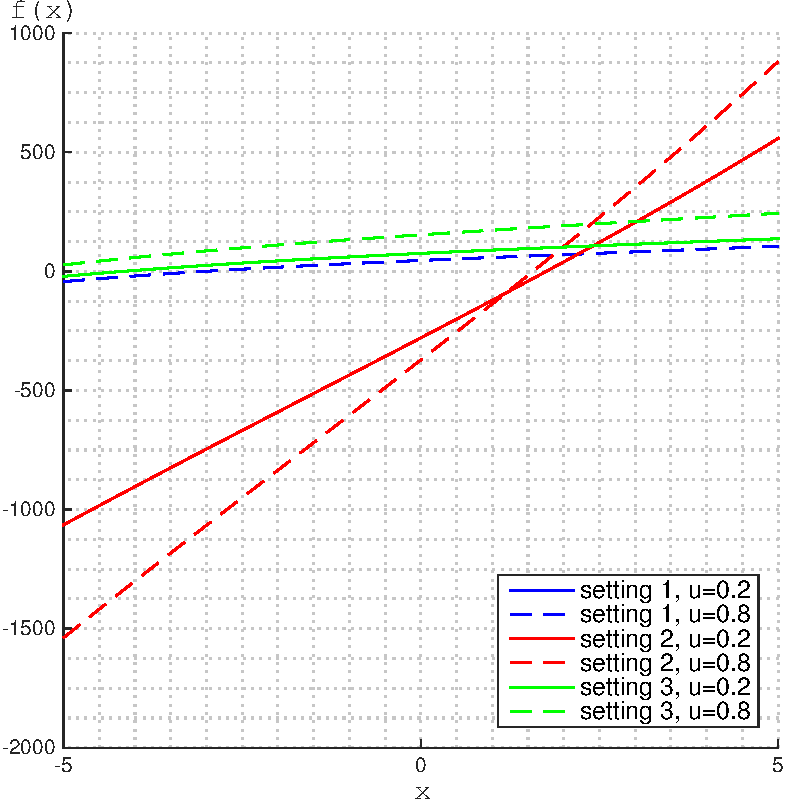
\includegraphics[width=0.6\textwidth]{graphics/fx.pdf}
	\caption{$f(x,u)$ within three different settings and u = 0.2 (solid) or u = 0.8 (dashed). In setting 1 (green) I use the \emph{charged} spot price vector, N=4 with two positively weighted assets in the spread and $\Sigma$ of type \emph{constant.} In setting 2 (blue) I use the \emph{descneding} spot price vector, N=20 with five positively weighted assets in the spread and $\Sigma$ of type \emph{alternating.} In setting 3 (red) I use the \emph{charged} spot price vector, N=10 with six positively weighted assets and $\Sigma$ of type \emph{descending}. Throughout I set $\sigma_k = 0.4, \; k=0,1,...,N$.}
	\label{fig:fx}
\end{figure}
Indeed $f(x)$ is a monotonic function such that \textit{fzero} is able to find a zero for given function. Denote that f(x) is not defined for $u=1$ and for $u=0$ there exists no zero as $f(x,0)=-K$. This poses a problem for the integrals which are defined on $u\in[0,1]$. To avoid this problem I limit the integration interval to $u\in[\delta u,1-\delta u],\; \delta u \rightarrow 0.$ In my implementation I set $\delta u = 10^{-12}.$ \\
Figure \ref{fig:ints} shows the two integrands in equation \ref{eq:ints}. 
\begin{figure}[h!]
	\centering
	\captionsetup{width=.6\linewidth}
	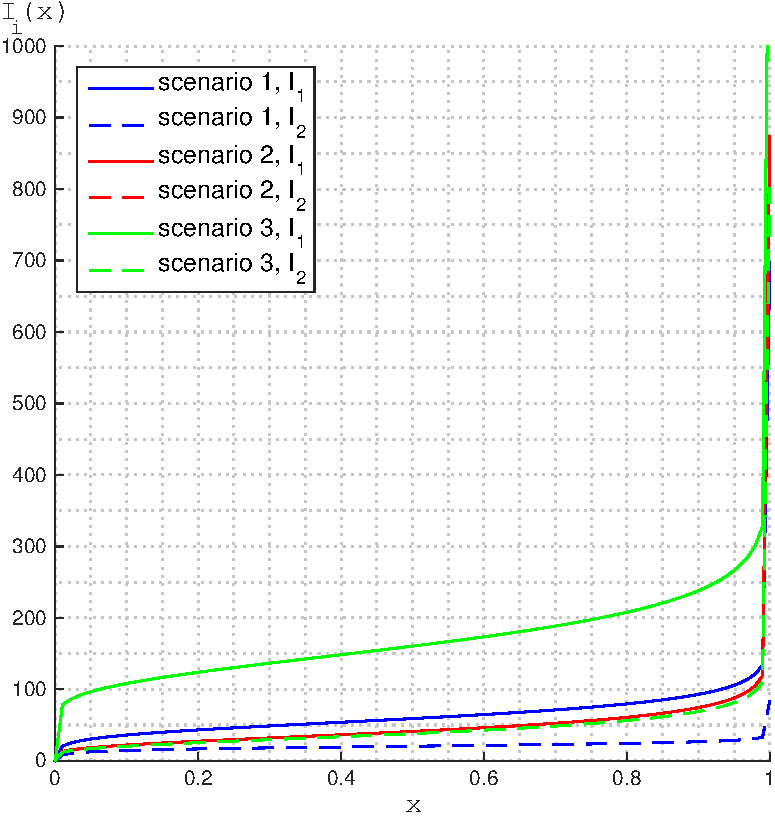
\includegraphics[width=0.6\textwidth]{graphics/ints_noTitle.pdf}
	\caption{Integrand 1 (solid) and 2 (dashed) from equation \ref{eq:ints}. I use the same three settings as in figure \ref{fig:fx}. Notice the instability of the integrands at the boundaries and the linear behaviour in the center region. This is an advantage for the adaptive Simpson's rule which can split up the interval more efficiently than a integration method using equal subintervals. }
	\label{fig:ints}
\end{figure}
To solve the integrals I considered two integration techniques, the adaptive Simpson's rule and the rectangle method. The adaptive Simpson's rule repeatedly splits an integral $I = \int_a^b g(x) dx$ in two subintervals $ I_l = \int_a^{\frac{b-a}{2}} g(x) dx$ and $I_r = \int_{\frac{b-a}{2}}^b g(x) dx$ until the termination criteria $|I-I_l-I_r| \leq \epsilon$ is met, whereas the integrals are numerically approximated according to the standard Simpson's rule. The rectangle method divides the interval (a,b) into $N$ equal subintervals of length $h=\frac{b-a}{N}$ and approximates the integral by adding up the areas of the $N$ rectangles under the curve. The rectangle method allows to precompute $F_{\mathbb{S}^{ic}|U=u}(K)$ for all subintervals once and reuse it in all three integrals. On the other hand the adaptive Simpson's rule might use less subintervals per integral but  this approach might evaluate $F_{\mathbb{S}^{ic}|U=u}(K)$ multiple times for the same subintervals as it is needed in all of the three integrands. Also rate of convergence until the termination criteria is met might be slow.\\
Clearly the accuracy and computing time of the two mentioned methods strongly depend on $\epsilon$ and $N$, respectively. A performance analysis based on convergence rate versus computing time shows that the adaptive Simpson's rule is outperforming the rectangle method. Also I conclude that setting $\epsilon = 10^{-5}$ is  a reasonable precision for the adaptive Simpon's rule.
\subsection{Run-time analysis}
\label{rt}
A plot will be enough to demonstrate that the SOB method (blue) is much faster than the HybMMICUB method (red). Figure \ref{fig:rt} shows the run-time of both methods measured within three different settings. The complexity of the SOB method is $\mathcal{O}(N^3)$ whereas the HybMMICUB method appears to behave linearly. But still the run-time of the SOB method is much shorter for a reasonable amount of underlyings (the SOB method is 1000 times faster for N=10 and 100 times faster for N=512). The experiment is run on a machine with a 1.8 GHz Intel Core i7 processor with 4GB of RAM,
\begin{figure}[h!]
	\centering
	\captionsetup{width=.6\linewidth}
	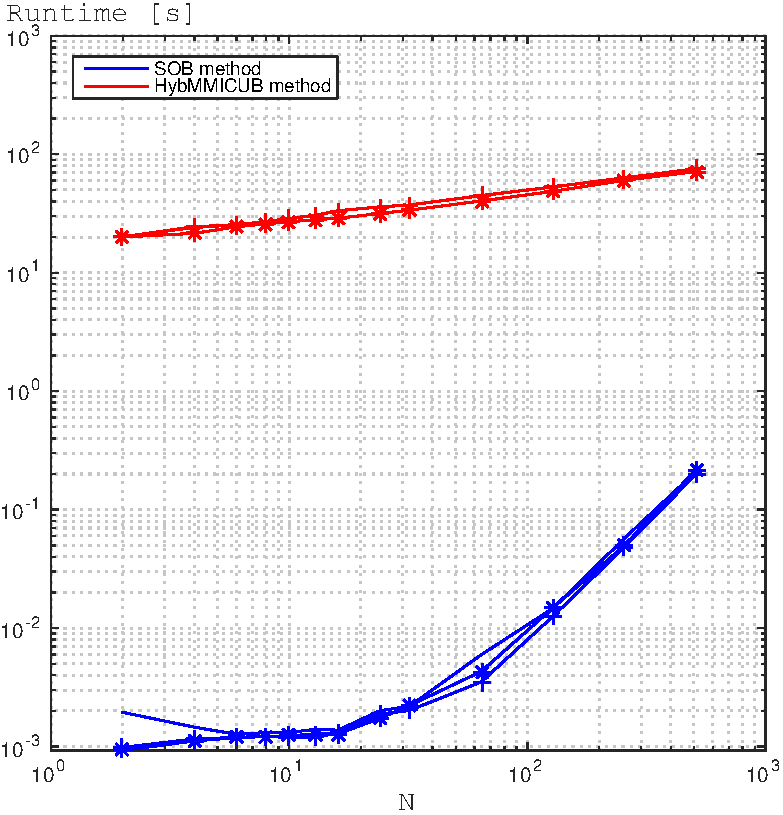
\includegraphics[width=0.6\textwidth]{graphics/runtime.pdf}
	\caption{Run-time of both pricing methods as a function of underlying assets N. I use three settings to validate the run-time of the methods. The complexity of 		the HybMMICUB method seems to be a linear function of N whereas the SOB method clearly shows its exponential behaviour.}
	\label{fig:rt}
\end{figure}

\subsection{Comparison of accuracy}
\label{sec:accuracy}
I now compare the accuracy of the second-order boundary approximation with the hybrid moment matching method associated to the improved comonotonic upper bound. To do that, I approximate the price of the options with Monte Carlo simulations and use it as as a rough comparison benchmark. To simulate the paths of the underlying assets I apply the Euler-Maruyama method. For each asset I generate 1'000'000 paths (respectively 500'000, if N big, which can lead to memory issues) having each path divided into 1000 (100, respectively) time-steps. I price every option five times to estimate the standard deviation of the Monte Carlo approximation. All following experiments run on the ETH Euler Cluster with a 2.4GHz Intel Core 2 Duo processor with 4GB of RAM. \\
First I replicate two experiments from [1] and from [2] to validate my implementations. Then I present my experiments for which I choose different correlation matrices and different volatility vectors. Some experiments are repeated while increasing the dimension from N=10 to N=50 or varying the volatility. In my last experiment I use a different structure of the spot prices and strikes. Throughout my experiments I set T=1 and r=5\%.\\

{\setstretch{1.5}
\textbf{Replication of Table 1 from \cite{sob} and Table 6 from \cite{hybmmicub} (Table 1 \& 2)}\\
}
In the first example I replicate the experiment from table 1 in \cite{sob}: I price a three-asset spread option with initial asset prices $S_0(0)=150, S_1(0) = 60$ and $S_2(0) = 50.$ The volatility vector is of type constant $\sigma = [0.3, 0.3, 0.3]$ ($\sigma = [0.6, 0.6, 0.6]$, respectively) and the correlation matrix is given by 
$$\Sigma =\begin{pmatrix}1 & 0.2 & 0.8\\ 
0.2 & 1 & 0.4\\
0.8 & 0.4 & 1 \end{pmatrix}.$$
Also I vary K from 30 to 50 with increment 5 and I set T =0.25 and r=5\%. The signs and the weights are equal $[1,-1,-1]$. From a comparison between my prices and the results from S.J. Deng, M. Li, J. Zhou I imply that I correctly implemented the SOB method although there are relative changes of order $1.5\times10^{-4}$. Looking at the prices calculated with the HybMMICUB method one can see that the SOB method is more accurate in this experiment. Taking my Monte Carlo estimate as a reference, in the HybMMICUB approximations occur relative errors up to $1.6 \times 10^{-2}$ whereas I have a maximal relative errors of $2.7\times10{-3}$ occuriing in the SOB approximations for K=50 and $\sigma = 60\%$. Again one can see that the SOB method is the fastest.\\
In table 2 I'm replicating the results from table 6 in \cite{hybmmicub}. It's noticeable that the SOB method completely mispriced the spread options. That is a result one could expect if you remember the condition $K\geq0$ from proposition \ref{prop:price} and you consider that all strike prices in this experiment are\ negative. My prices slightly deviate from the results from G. Deelsra, A. Petkovic and M.Vanmaele. There are maximal relative changes of order $5\times10^{-2}$. Such changes can happen because there is much freedom in the implementation, namely the choice of integration scheme, how you cope with the boundaries of the integrals and how the zero finding problem is solved. The relative errors range from $5\times10^{-2}$ (K=-60) to $11\times10^-{2}$ (K=-5).\\
In paper \cite{sob} and \cite{hybmmicub} the authors test their approximation methods solely on spread options with strictly one asset positively accounted in the spread. In my experiments I strictly use five assets with a positive sign while varying the number of assets between N=10 to N=50.\\

\newpage
{\setstretch{1.5}
\textbf{Setting: Descending Volatilities (Table 3)}\\
}
In this experiment I am applying a different volatility to each asset. For N = 10 the HybMMICUB method constantly produces relative pricing errors  $7\times10^{-2}$ whereby the SOB errors range from $5\times10^{-2}$ (K=50)  to $15\times10^{-2}$ (K=90). Also in other experiments one will see that errors of the SOB approximations continuously increase as the strike price K increases. For N=50 the SOB method completely mispriced the basket-spread options. Surprisingly the relative errors of the HybMMICUB method reduce for the case N=50. \\

{\setstretch{1.5}
\textbf{Setting: Alternating Correlation Matrix (Tables 4 \& 5) and Descending Correlation Matrix (Tables 6 \& 7)}\\
}
Here one can recognize that in both settings with N=50 the SOB method produces poor approximations. The HybMMICUB delivers reasonable prices with relative errors of the order $5\times10^{-2}$. The accuracy of the approximations is slightly reduced in the case of $\sigma=60\%.$\\

{\setstretch{1.5}
\textbf{Setting: Descending Spot Prices (Table 8)}\\
}
The 5 assets positively accounted in the spread have spot prices [100, 90, ..., 60] and the other 5 spot prices are given by the vector [50, ..., 10]. The strike prices vary from 100 to 180 with increment 20. Meaning that at time zero the option is definitely in the money. In the table one can observe that for $\sigma = 30\%$ the SOB method delivers accurate results whereas the approximations of the HybMMICUB method are favorable in the case of $\sigma = 60\%.$

\newpage
\section{Conclusion}
\label{sec:conclusion}
I started by presenting both the second-order boundary method and the hybrid moment matching method associated to the improved comonotonic upper bound. Based on the derivation of the methods it is clear that the SOB method is more straightforward to implement than HybMMICUB. Solely involving arithmetic operations, the SOB method is up to 1000 times faster than the latter. Consider that the SOB method allows further optimization if pricing options including the same assets but varying strike prices: computational costly operations such as calculating the square of a matrix or the few matrix-matrix multiplications involved are independent of K could be prestored and reused.\\
Both methods can be very accurate (taking into account the results from \cite{sob} and \cite{hybmmicub}) if applied on spread options with strictly one positively weighted asset, whereas the SOB method is slightly more accurate (table 1).  But while extending the experiments to basket-spread options including more positively weighted assets it becomes clear that the SOB method is not anymore applicable if the total number of assets increases to N = 50 (relative error >20\%). Looking at spread options involving N=10 assets one can see that the accuracy of the SOB method correlates with the strike price. If the strike price is low (at time zero the option is close to at-the-money) the SOB approximation outperforms the HybMMICUB, but for out-of-the-money options the HybMMICUB approximation yields more accurate results. I conclude that the HybMMICUB method is more stable in terms of the spread characteristics and market conditions such as correlations and volatilities. Also note that the HybMMCUB overpriced all options in my experiments and it truly is an upper bound which is an asset in estimating basket-spread options.

\newpage
\begin{thebibliography}{1}
\bibitem{sob} 
S.J. Deng, M. Li, J. Zhou.
\textit{Multi-asset Spread Option Pricing and Hedging.}
October 29, 2007. School of Industrial and Systems Engineering, Georgia Institute of Technology, Atlanta.

\bibitem{hybmmicub} 
G. Deelstra, A. Petkovic, M. Vanmaele.
\textit{Pricing and Hedging Asian Basket Spread Options.}
2010. Journal of Computational and Applied Mathematics 233 2814-2830.

\bibitem{sob2} 
S.J. Deng, M. Li,  J. Zhou. 
\textit{Closed-form approximations for spread option prices and Greeks.} 2006.
Available at http://ssrn.com/abstract=952747.

\bibitem{cd} 
Carmona, R., V. Durrleman. 
\textit{Generalizing the Black-Scholes formula to multivariate contigent claims.} 2005. Journal of Computational Finance, 9, 42-63.

\bibitem{li}
M. Li.
\textit{The impact of return nonnormality on exchange options.} 2007.
Journal of Futures Markets, working paper, forthcoming.

\bibitem{pearson}
Pearson, N. 
\textit{An efficient approach for pricing spread options.} 1995. Journal of Derivatives, Fall, 76-91.

\end{thebibliography}

\newpage
\section*{Appendix: Numerical Results}
\label{sec:appendix}

\captionsetup{skip=0pt}
\begin {table}[H]
\caption {Replication of Table 1 in [1]} 
\begin{center}
\begin{tabular}{c|c c c c|c c c c}
\hline
\multicolumn{1}{c|}{} & \multicolumn{4}{|c|}{$\sigma$=30\%} & \multicolumn{4}{|c}{$\sigma$=60\%} \\ 
\hline
  \textbf{K} & \textbf{SOB} & \textbf{Hyb}	& \textbf{MC} & \textbf{S.E.} & \textbf{SOB} & \textbf{Hyb} & \textbf{MC} & \textbf{S.E.}\\
  30 &	13.574 & 13.708 & 13.574 & 0.009 &  20.19 & 20.37  & 20.22 & 0.04 \\
  35 & 10.356 & 10.465 & 10.354 & 0.009 & 17.46  & 17.64 &17.49 & 0.04  \\
 40 & 7.660 & 7.754 & 7.658 & 0.008 & 15.01  & 15.12  & 15.04 & 0.03  \\
 45 & 5.490 & 5.575 & 5.487  & 0.007 & 12.84  &13.03  &12.87  & 0.03\\
 50 & 3.813 & 3.892 & 3.812  & 0.005 & 10.92  & 11.12 &10.95  &0.03 \\
\hline
Time [s] & 0.02028 & 26.302 & 243.34 & & 0.0009&  32.737 & 259.82 & \\
\hline
\end{tabular}
\\[8pt]
\caption*{$a=[1,-1,-1], S_0(0)=150, S_1(0) = 60, S_2(0) = 50, \sigma_k = 0.3, (\sigma_k = 0.6),\rho_{12} = 0.2, \rho_{13} = 0.8, \rho_{23} = 0.4, T = 0.25, r=0.05.$}
\end{center}
\end{table}

\begin {table}[H]
\caption {Replication of Table 6 in [2]} 
\begin{center}
\begin{tabular}{c|c c c c}
\hline
\multicolumn{1}{c|}{} & \multicolumn{4}{|c}{} \\ 
\hline
  \textbf{K} & \textbf{SOB} & \textbf{Hyb} & \textbf{MC} & \textbf{S.E.}\\
  -5 & 2.738	& 1.602	& 1.437    &  0.003\\
-10 & 4.225	& 2.499	& 2.278    & 0.004\\
-20 & 8.159	& 5.309	& 4.949    & 0.006\\
-30 & 12.178	& 9.665	& 9.124& 0.009\\
-40 & 15.454	& 15.559	& 14.77 & 0.012\\
-50 & 18.950	& 22.771	& 21.68 & 0.016\\
-60 & 22.948	& 30.985	& 29.52 & 0.019\\
\hline
Time [s] & 0.0151 & 11.869 & 248.59 & \\
\hline
\end{tabular}
\\[8pt]
\caption*{$a=[1,-1,-1, -1], S_0(0)=100, S_1(0) = 60, S_2(0) = 40, S_3{0} = 30, \sigma = [0.16, 0.23, 0.32, 0.43], \rho_{12} = 0.2, \rho_{13} = 0.8, \rho_{23} = 0.4, T = 1, r=0.05.$}
\end{center}
\end{table}

\begin {table}[H]
\caption {Descending Volatilities, 10 Assets} 
\begin{center}
\begin{tabular}{c|c c c c|c c c c}
\hline
\multicolumn{1}{c|}{} & \multicolumn{4}{|c|}{N = 10} & \multicolumn{4}{|c}{N=50} \\ 
\hline
  \textbf{K} & \textbf{SOB} & \textbf{Hyb} & \textbf{MC} & \textbf{S.E.} & \textbf{SOB} & \textbf{Hyb} & \textbf{MC} & \textbf{S.E.}\\
50 &	54.17& 60.52 	& 56.79 & 0.06 & 84.65 & 133.42 & 125.94 & 0.11 \\
60 & 46.51	& 53.39 	& 49.94 & 0.06   & 79.56  & 128.90 & 121.68 & 0.10  \\
70 & 39.72	& 46.96	& 43.81 & 0.06  & 74.73 & 124.54 & 117.57 & 0.10\\
80 & 33.77	& 41.20 	& 38.37 & 0.06  & 70.13  & 120.34 & 113.60 & 0.10  \\
90 & 28.59& 36.10	& 33.57  & 0.06  & 65.77 & 116.26 & 109.78 &0.10\\
\hline
Time [s] & 0.0223 & 38.796 & 902.11 & & 0.0184 & 32.760 & 419.13 \\
\hline
\end{tabular}
\\[8pt]
\caption*{5 assets with positive sign, $S_0(0)=10(N+1), S_{k\geq1}(0) = 10, \sigma = [0.6, ..., 0.1]$ evenly spaced, $\rho_{i\neq j} = 0.4, T = 1, r=0.05.$}
\end{center}
\end{table}

\begin {table}
\caption {Alternating Correlation Matrix $\Sigma$, 10 Assets} 
\begin{center}
\begin{tabular}{c|c c c c|c c c c}
\hline
\multicolumn{1}{c|}{} & \multicolumn{4}{|c|}{$\sigma$=30\%} & \multicolumn{4}{|c}{$\sigma$=60\%} \\ 
\hline
  \textbf{K} & \textbf{SOB} & \textbf{Hyb} & \textbf{MC} & \textbf{S.E.} & \textbf{SOB} & \textbf{Hyb} & \textbf{MC} & \textbf{S.E.} \\
50 &	52.46&55.30	&52.56  &0.06  &54.19  &59.25&55.80&0.05  \\
60 & 	43.09&45.74 	&43.43  &0.05  &46.40  &51.85&48.71&0.05  \\
70 & 	34.12&36.79 	&34.87  &0.05  &39.42  &45.22&42.38&0.04  \\
80 & 	25.95&28.73 	&27.20  &0.05  &33.29  &39.33&36.81&0.04  \\
90 &  18.95&21.82 	&20.63  &0.05  &27.99  &34.16&31.94&0.03  \\
\hline
Time [s] & 0.0222&30.853 &845.19 & &0.0206  &40.376& 845.67& \\
\hline
\end{tabular}
\\[8pt]
\caption*{5 assets with positive sign, $S_0(0)=10(N+1), S_{k\geq1}(0) = 10, \sigma_k = 0.3 (\sigma_k = 0.6), \rho_{i\neq j} = 0.4\times-1^{i+j}, T = 1, r=0.05.$}
\end{center}
\end{table}

\begin {table}
\caption {Alternating Correlation Matrix $\Sigma$, 50 Assets} 
\begin{center}
\begin{tabular}{c|c c c c|c c c c}
\hline
\multicolumn{1}{c|}{} & \multicolumn{4}{|c|}{$\sigma$=30\%} & \multicolumn{4}{|c}{$\sigma$=60\%} \\ 
\hline
  \textbf{K} & \textbf{SOB} & \textbf{Hyb}	& \textbf{MC} & \textbf{S.E.} & \textbf{SOB} & \textbf{Hyb} & \textbf{MC} & \textbf{S.E.}\\
50 &	57.86&80.52 	& 76.37  & 0.02 & 73.95  &126.07 &118.99 &0.17 \\
60 & 	50.46& 74.36& 70.53 & 0.02&67.11 &121.22 & 114.42&0.17 \\
70 & 43.60& 68.55& 65.03& 0.02& 60.38&116.56&110.03&0.17\\
80 & 	37.33& 63.08& 59.85& 0.02&53.85&112.08&105.82&0.16 \\
90 & 31.67& 57.95& 54.10& 0.02&47.56&107.78&101.78&0.12\\
\hline
Time [s] & 0.0176 &32.5937 & 528.71 & &0.0232 &40.930 & 569.28 & \\
\hline
\end{tabular}
\\[8pt]
\caption*{5 assets with positive sign, $S_0(0)=10(N+1), S_{k\geq1}(0) = 10, \sigma_k = 0.3 (\sigma_k = 0.6), \rho_{i\neq j} = 0.4\times-1^{i+j}, T = 1, r=0.05.$}
\end{center}
\end{table}

\begin {table}
\caption {Descending Correlation Matrix $\Sigma$, 10 Assets} 
\begin{center}
\begin{tabular}{c|c c c c|c c c c}
\hline
\multicolumn{1}{c|}{} & \multicolumn{4}{|c|}{$\sigma$=30\%} & \multicolumn{4}{|c}{$\sigma$=60\%} \\ 
\hline
  \textbf{K} & \textbf{SOB} & \textbf{Hyb}	& \textbf{MC} & \textbf{S.E.} & \textbf{SOB} & \textbf{Hyb} & \textbf{MC} & \textbf{S.E.} \\
50 &	52.47	&	55.53	&	52.75	& 0.01	&	54.33	&	61.28	&	57.56 &	0.02 \\
60 & 	43.10	& 	46.21	& 	43.83 	& 0.01  &46.33 & 54.14 & 50.70& 0.02 \\
70 & 34.05 	& 37.51&35.52& 0.01& 39.06&47.68& 44.53 &0.03 \\
80 & 	25.68	&  29.69&28.07&0.01& 32.57& 41.87&39.07&0.03 \\
90 & 18.38 	& 22.93& 21.66 &0.01 & 26.91 &36.70 & 34.16 & 0.03 \\
\hline
Time [s] &0.0205 & 26.590 & 905.52 & &0.0200 &34.706& 897.07 & \\
\hline
\end{tabular}
\\[8pt]
\caption*{5 assets with positive sign, $S_0(0)=10(N+1), S_{k\geq1}(0) = 10, \sigma_k = 0.3 (\sigma_k = 0.6), \rho_{i\neq j} = \frac{1}{i+j}, T = 1, r=0.05.$}
\end{center}
\end{table}

\begin {table}
\caption {Descending Correlation Matrix $\Sigma$, 50 Assets} 
\begin{center}
\begin{tabular}{c|c c c  c|c c c c}
\hline
\multicolumn{1}{c|}{} & \multicolumn{4}{|c|}{$\sigma$=30\%} & \multicolumn{4}{|c}{$\sigma$=60\%} \\ 
\hline
  \textbf{K} & \textbf{SOB} & \textbf{Hyb}	& \textbf{MC}& \textbf{S.E.} & \textbf{SOB} & \textbf{Hyb} & \textbf{MC}& \textbf{S.E.} \\
50 &73.95&126.07&118.99&0.17& 92.38 &  150.20&141.99 &0.16  \\
60 &67.11&121.22&114.42&0.17& 87.20&  145.67&137.71 &0.17\\
70 &60.38&116.56&110.03&0.17& 82.27& 141.27 & 133.56 &0.17\\
80 &53.85&112.08&105.82& 0.16& 77.57& 137.01& 129.53 &0.17\\
90 &47.60&107.78&101.78& 0.16& 73.11&  132.87& 125.63 &0.17\\
\hline
Time [s] &0.0176 &32.59 &528.72 & &0.0172 &27.478&488.82 \\
\hline
\end{tabular}
\\[8pt]
\caption*{5 assets with positive sign, $S_0(0)=10(N+1), S_{k\geq1}(0) = 10, \sigma_k = 0.3 (\sigma_k = 0.6), \rho_{i\neq j} = \frac{1}{i+j}, T = 1, r=0.05.$}
\end{center}
\end{table}

\begin {table}
\caption {Descending Spot Prices, 10 Assets} 
\begin{center}
\begin{tabular}{c|c c c c|c c c c}
\hline
\multicolumn{1}{c|}{} & \multicolumn{4}{|c|}{$\sigma$=30\%} & \multicolumn{4}{|c}{$\sigma$=60\%} \\ 
\hline
  \textbf{K} & \textbf{SOB} & \textbf{Hyb}	& \textbf{MC}& \textbf{S.E.} & \textbf{SOB} & \textbf{Hyb} & \textbf{MC} & \textbf{S.E.} \\
100 &40.96&43.81&41.69& 0.05& 56.10& 62.85&59.67 & 0.11\\
120 &28.46&30.61& 29.12& 0.05&46.18& 52.39&49.73&0.10\\
140 &19.06&20.43& 19.43& 0.04& 38.16&43.51&41.30&0.10\\
160 &12.45&13.08& 12.44& 0.03 & 31.79&36.05& 34.22& 0.09 \\
180 &7.98& 8.08&7.69 & 0.03& 26.72&29.82&28.31&0.09\\
\hline
Time [s]& 0.0190&34.446& 796.64 & & 0.0209& 49.270&815.59 & \\
\hline
\end{tabular}
\\[8pt]
\caption*{5 assets with positive sign, N=10 assets, $S_k(0)=10(N+1-k), \sigma_k = 0.3 (\sigma_k = 0.6), \rho_{i\neq j} = 0.4, T = 1, r=0.05.$}
\end{center}
\end{table}

\end{document}





